In this section, we introduce \verb!Citadel!. We start with an overview of the protocol, its elements, and its use cases. Then, we introduce the main element required by our solution: a private NFT model for Dusk. Finally, we detail our novel SSI system, \verb!Citadel!.

\subsection{Overview}

In this section, we describe a novel protocol for authenticating in several services but preserving at the very same time our privacy. Imagine we want to buy a ticket for a concert. Nowadays, what we would do in most cases is to buy the ticket using a web page that will get information about our browser, our credit card, our bank account, ourselves... Moreover, they will charge us a fee for the ticket management service, and probably they will charge a fee to the concert promotor as well. Furthermore, as soon as we show the ticket to the concert, they will be able to link our image to the information previously gathered.

Using \verb!Citadel!, we can do much better. In particular, we want to buy a license (a.k.a. a right) to use some service (e.g. the ticket of the example above is a license, to be used in a concert, which is a service) without leaking any information about us. Furthermore, we want to use such a service as many times as permitted by the SP, without them being able to link our activity, or learn our identity. Moreover, we want a decentralized system that does not rely on third parties to manage our identities and licenses.

To achieve the aforesaid features, we first rely on Dusk Network as the decentralized framework that our solution is based. Then, we need a way to privately share assets among users of the Dusk Network. For this reason, in Section \ref{sec:privatenft} we design a novel and private NFT model for Dusk. Finally, we need a way to anonymously prove ownership of our acquired licenses (i.e. the NFTs), so we introduce our solution in Section \ref{sec:citadel}.

\subsection{A Private NFT Model for Dusk}
\label{sec:privatenft}

As described in Section \ref{sec:buildingblocks}, coins in Dusk are represented as notes, and they can be either transparent note ($\type = 0$), or obfuscated note ($\type = 1$). Here we introduce two new types of notes: transparent NFT note ($\type = 2$) and obfuscated NFT note ($\type = 3$). 

As stated previously, a user willing to spend Dusk notes needs to mint new notes while nullifying the old ones. Like this, a user can spend one note, and create a new note for the receiver, and another one with the change for themselves. When willing to mint a new NFT, a user will need to execute the minting contract where a Dusk note will be used to pay for the contract gas (and thus, it will be nullified), and a new note will be created to receive the change. Additionally, a new NFT note will be created. The creation of an NFT note does not need to be part of the ZKP circuit, as it is not involved in the balance to be verified. As such, it is enough to include the new NFT note in the transaction. A note representing an NFT contains the same data as other notes do, but in this case, what before was the note value in Dusk coins $v$, now is the $\nftpayload$ of the NFT. To mint a new note, we first compute the note public key $\npk$ and the value $R$ of the receiver as described in Section~\ref{sec:protocol-keys}, plus the symmetric key $\kdh$. Then, we set the parameters of each new NFT note $\mathsf{N}$ by executing a function 
\[\mintnft(\npk, R, \nftpayload, \kdh)\]
whose workflow is described in Algorithm \ref{alg:mintnft}.

\begin{algorithm}
\SetAlgoLined
\textbf{Inputs:} \par
$(\npk, R)$: the public note key of the receiver $\npk$ and the related value $R$.\\
$\nftpayload$: a value being the desired content of our NFT note $\Note{}$.\\
$\ksym$: a symmetric encryption key.\break

\textbf{Algorithm:}
	\begin{enumerate}
		\item Set the type of note.
		\begin{itemize}
			\item If the NFT note is transparent, set $\type = 2$.
			\item If the NFT note is obfuscated, set $\type = 3$.
		\end{itemize}
		\item Set a nonce for the encryption.
		\begin{itemize}
			\item If $\type = 2$, set $\nonce = 0$.
			\item If $\type = 3$, set $\nonce \leftarrow \F_t$.
		\end{itemize}
		\item Encrypt the $\nftpayload$.
		\begin{itemize}
			\item If $\type = 2$, then set $\enc = \nftpayload$.
			\item If $\type = 3$, then 
			$\enc = \Enc_{\ksym} (\nftpayload; \nonce)$,
			where $\Enc()$ is a symmetric encryption function. 
		\end{itemize}
		\item Set the new NFT note to \[\Note = \{\type, \enc, \nonce, R, \npk\}.\]
	\end{enumerate}
	\caption{Minting algorithm for private NFTs.}
	\label{alg:mintnft}
\end{algorithm}

As described previously, users willing to spend notes have to nullify them, a process that involves providing a ZKP whose circuit computes the hash of the note. In this process, the parameter $\type$ is set to private, as it is not relevant information for the protocol. \textbf{It is of paramount importance} to notice that after deploying this model, this parameter has to be public. Otherwise, an adversary could spend an NFT note pretending to be spending a regular note and would be able to create huge amounts of money out of the blue.

On the other hand, and as described in this section, the changes in the whole protocol are minimal. As such, deploying our model to the current system should be trivial.

% Furthermore, it is interesting to provide a way to prove ownership of a given NFT. Let us have our prover $\mathcal{P}$ willing to prove ownership of an NFT to a verifying party $\mathcal{V}$. A challenge-response protocol for achieving this purpose is described as follows.

% \begin{protocol}{Proving ownership of an NFT note.}
% \label{pro:citadel}
% \textbf{Environment:} \par
% A prover $\mathcal{P}$ knowing $\nsk$ willing to prove ownership of an NFT with note public key $\npk$. \\
% A verifying party $\mathcal{V}$ that wants to be convinced of $\mathcal{P}$'s statement. \\

% \\
% \textbf{Protocol:}
% 	\begin{enumerate}
% 		\item $\mathcal{V} \rightarrow \mathcal{P}$ : $r \leftarrow \F_t$ \$
% 		\item $\mathcal{P} \rightarrow \mathcal{V}$ : $\sig = \sign_{\nsk}(r)$ 
% 		\item $\mathcal{V} \rightarrow$  : $1/0 \leftarrow \verify_{\npk}(\sig, r)$ 
% 	\end{enumerate}
% \end{protocol}


\subsection{Description of Citadel}
\label{sec:citadel}

Now, we are going the introduce all the details about \verb!Citadel!. Then, we will detail its security analysis, and finally, we will perform some experiments in order to get benchmarks of the protocol.

\subsubsection{Protocol Details}

Let us have a user willing to pay a service provider SP for a license to use their service, and willing to anonymously prove ownership of this license afterward. First, the user will execute a payment in the Dusk Network addressed to the SP, including into the transaction the required information to receive the license. Upon receiving the payment, the SP will send back a license to the user, using the same Blockchain. In order to use the license, the user will have to call a smart contract deployed in the Dusk Network, called the \textit{license contract}. Essentially, the user will provide a proof that demonstrates that they own a valid license, the license contract will verify the proof, and will append a license nullifier to a Merkle tree of nullifiers. By means of a session cookie included in the same contract call, and addressed to the SP, the user will be able to request the service using an off-chain and secure channel. The workflow is depicted in Figure \ref{fig:protocol}, and described with full details in the following protocol.

\begin{protocol}{Citadel.}
\label{pro:citadel}
\textbf{Environment:} \par
A Service Provider SP offering a service, and publicly sharing its public key $\pk_{\SP}$. \\
A user willing to use a service provided by the SP. \\
The Dusk Network Blockchain.

\\
\textbf{Protocol:}
	\begin{enumerate}
		\item (\textbf{user}) $\mathsf{send\_note\_license\_req}$ : Compute a note public key $(\npk_{\user}, R_{\user})$ belonging to the user, using the user's own public key, and also an additional key $\ksym_{\user} = \hp(\npk_{\user}, \nsk_{\user})$, by computing first the user's $\nsk_{\user}$. Then, send the required amount of Dusk coins to the SP, in order to pay for the service. Into the same transaction, send an NFT to the SP using the function $\mintnft(\npk_{\SP}, R_{\SP}, \nftpayload, \kdh)$, whose arguments are computed as follows:
		\begin{itemize}
			\item $(\npk_{\SP}, R_{\SP})$ is the SP's note public key, computed through his public key $\pk_{\SP}$.
			\item $\nftpayload = (\npk_{\user}, R_{\user}, \ksym_{\user})$.
			\item $\kdh$ is computed using the SP's public key.
		\end{itemize}

		\item (\textbf{SP}) $\mathsf{get\_note\_license\_req}$ : Continuously check the network for incoming license requests. Upon receiving the payment from a user, define a set of attributes $attr$ representing the license, and compute a digital signature as follows:

		$$\lsig= \sign_{\sk_{\SP}}(\npk_{\user}, \attr)$$

		\item (\textbf{SP}) $\mathsf{send\_note\_license}$ : Set the $\nftpayload = \{\lsig, \attr\}$, and send the license to the user using the function $\mintnft(\npk_{\user}, R_{\user}, \nftpayload, \ksym_{\user})$.

		\item (\textbf{user}) $\mathsf{get\_note\_license}$ : Receive the note containing the license. 

		\item (\textbf{user}) $\mathsf{call\_nullify\_license}$ : When desiring to use the license, nullify it by executing a call to the license contract. The following steps are performed:

		\begin{itemize}
			\item The user sets a session cookie $\stoken = (\mathsf{s_0}, \mathsf{s_1}, \mathsf{s_2}) \leftarrow \F_t$.
			\item The user creates a new NFT note where $\nftpayload = \stoken$, and the SP is the receiver.
			\item The user issues the transaction that includes the NFT described in the previous step, by calling the license contract. In this case, the \textsf{tx\_proof} is computed as done in the standard Phoenix model, but into the same circuit, the circuit depicted in Figure \ref{fig:circuit_prove_nft} is appended.
			\item The network validators will execute the smart contract, which verifies the proof. Upon success, the NFT note will be forwarded, and the license nullifier $\lnullifier$ will be added to the Merkle tree of nullifiers.
		\end{itemize}

		\item (\textbf{SP}) $\mathsf{get\_note\_session\_cookie}$ : Receive a note containing the session cookie $\stoken$.

		\item (\textbf{user}) $\mathsf{req\_service}$ : Request the service to the SP, establishing communication using a secure channel, and providing the tuple $(\mathsf{tx\_hash}, \pk_{\SP}, \attr, c, \stoken)$.

		\item (\textbf{SP}) $\mathsf{grant\_service}$ : Grant or deny the service upon verification of the following steps:

		\begin{itemize}
			\item Check whether or not the values $(\attr, \pk_{\SP}, c)$ are correct.
			\item Check whether or not the openings $((\pk_{\SP}, \mathsf{s_0}), (\attr, \mathsf{s_1}), (c, \mathsf{s_2}))$ match the commitments $\com_0^{hash}, \com_1, \com_2$ found in the transaction $\mathsf{tx\_hash}$.
		\end{itemize}

	\end{enumerate}
\end{protocol}

\begin{figure}[h]
	\centering
		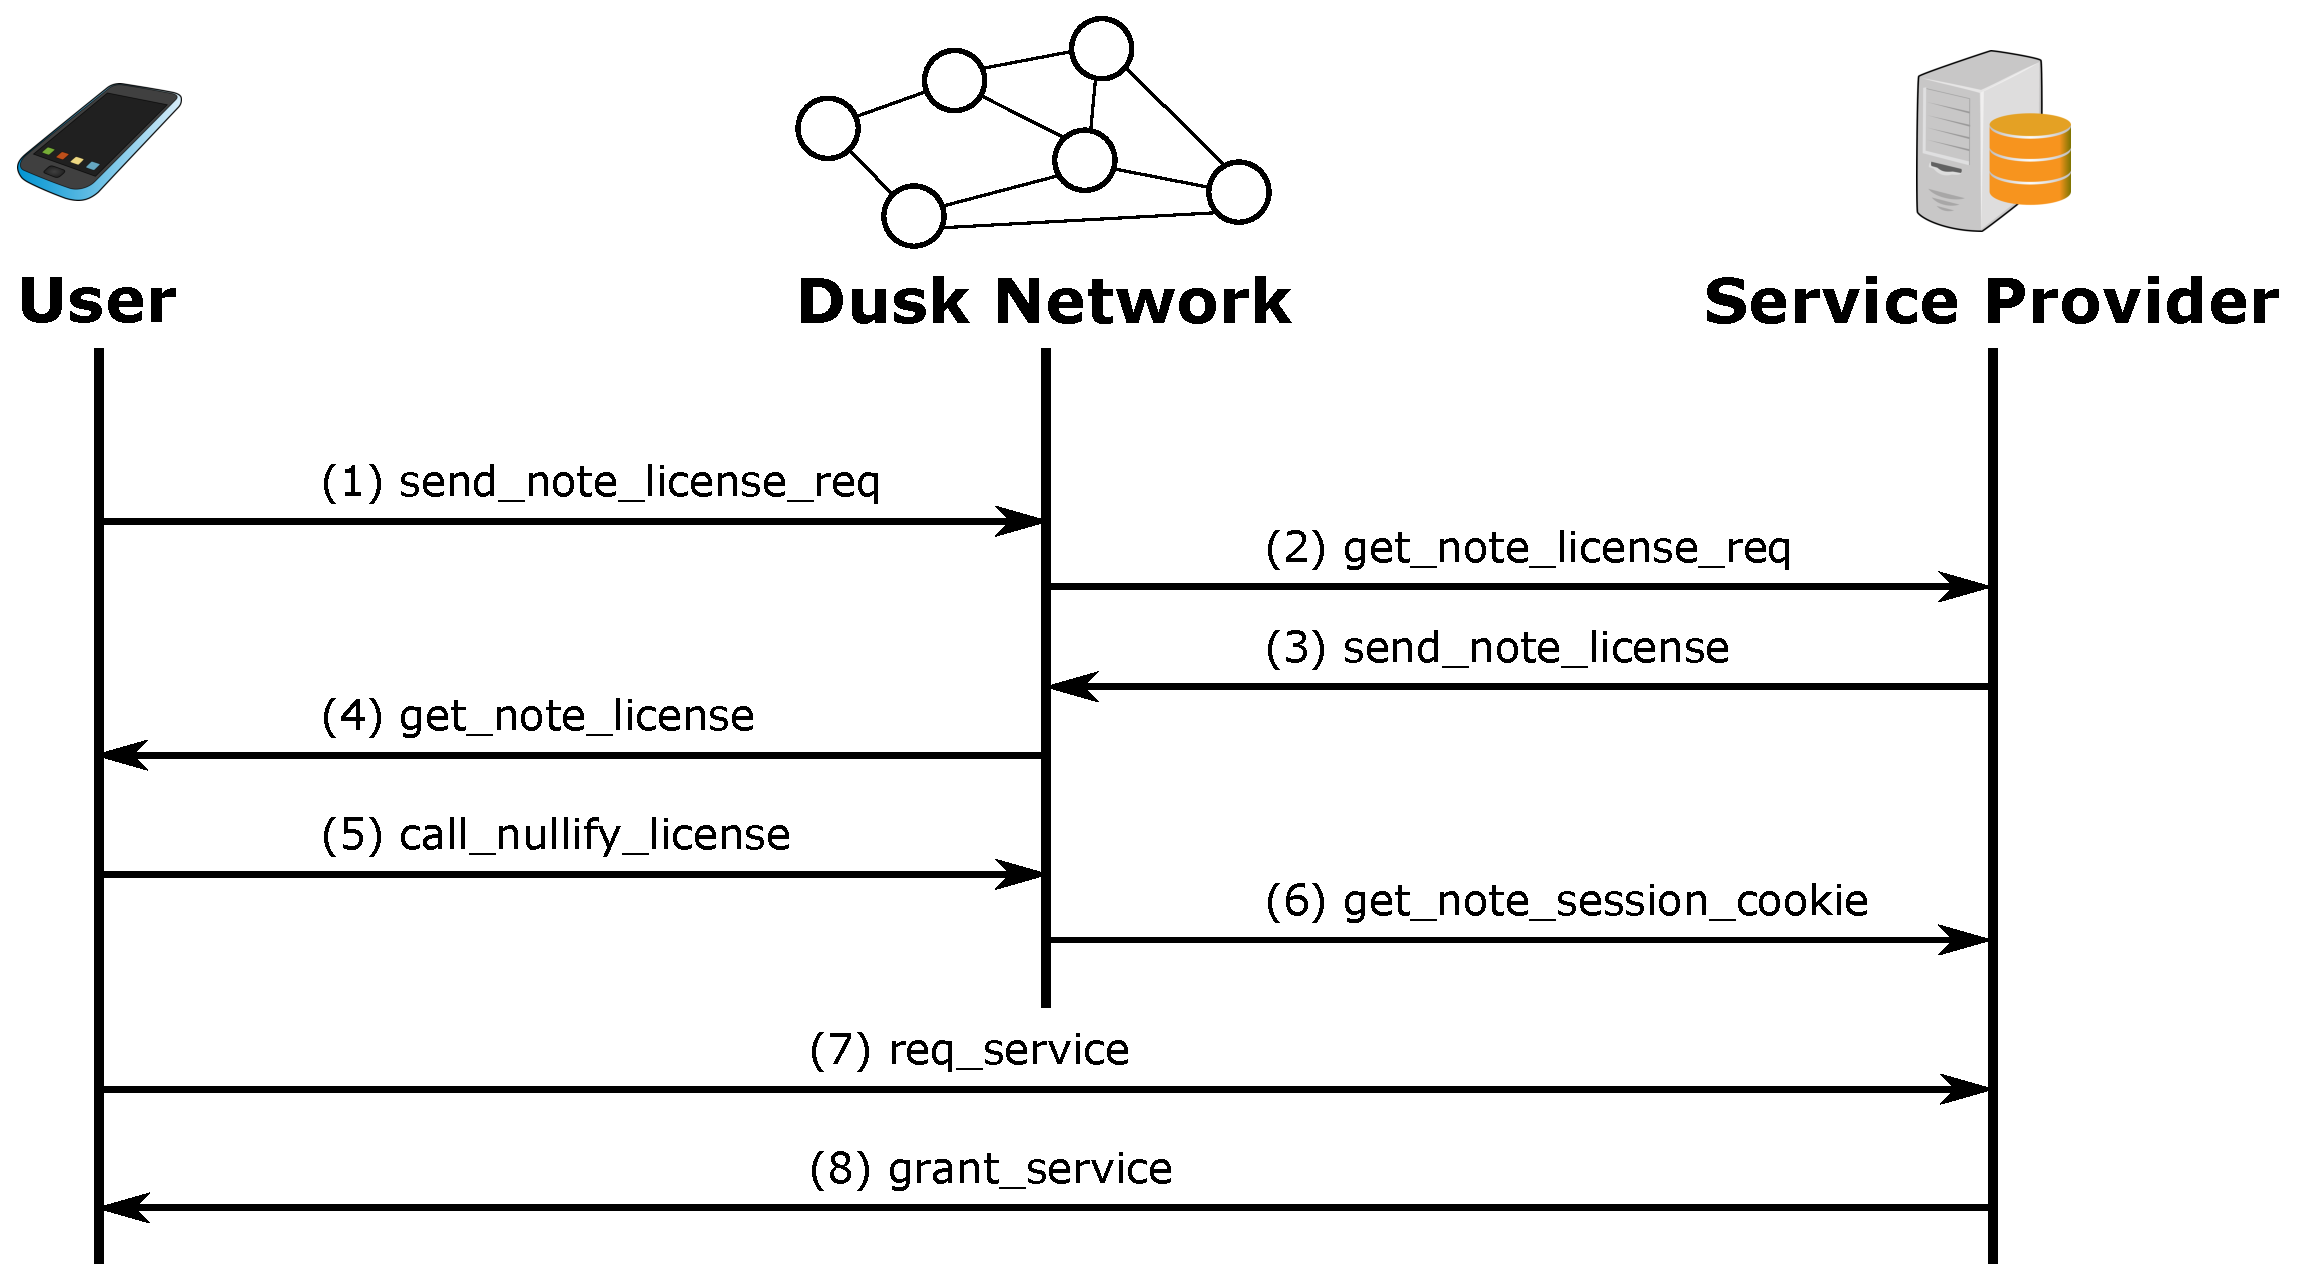
\includegraphics[width=390pt,draft=false]{images/protocol.eps}
	\caption{Overview of the protocol messages exchanged between the user, the Dusk Network, and the SP.}
	\label{fig:protocol}
\end{figure}

\begin{figure}[h]
	\centering
	\setlength{\fboxsep}{5pt}%
	\setlength{\fboxrule}{0.3pt}%
	\fbox{
		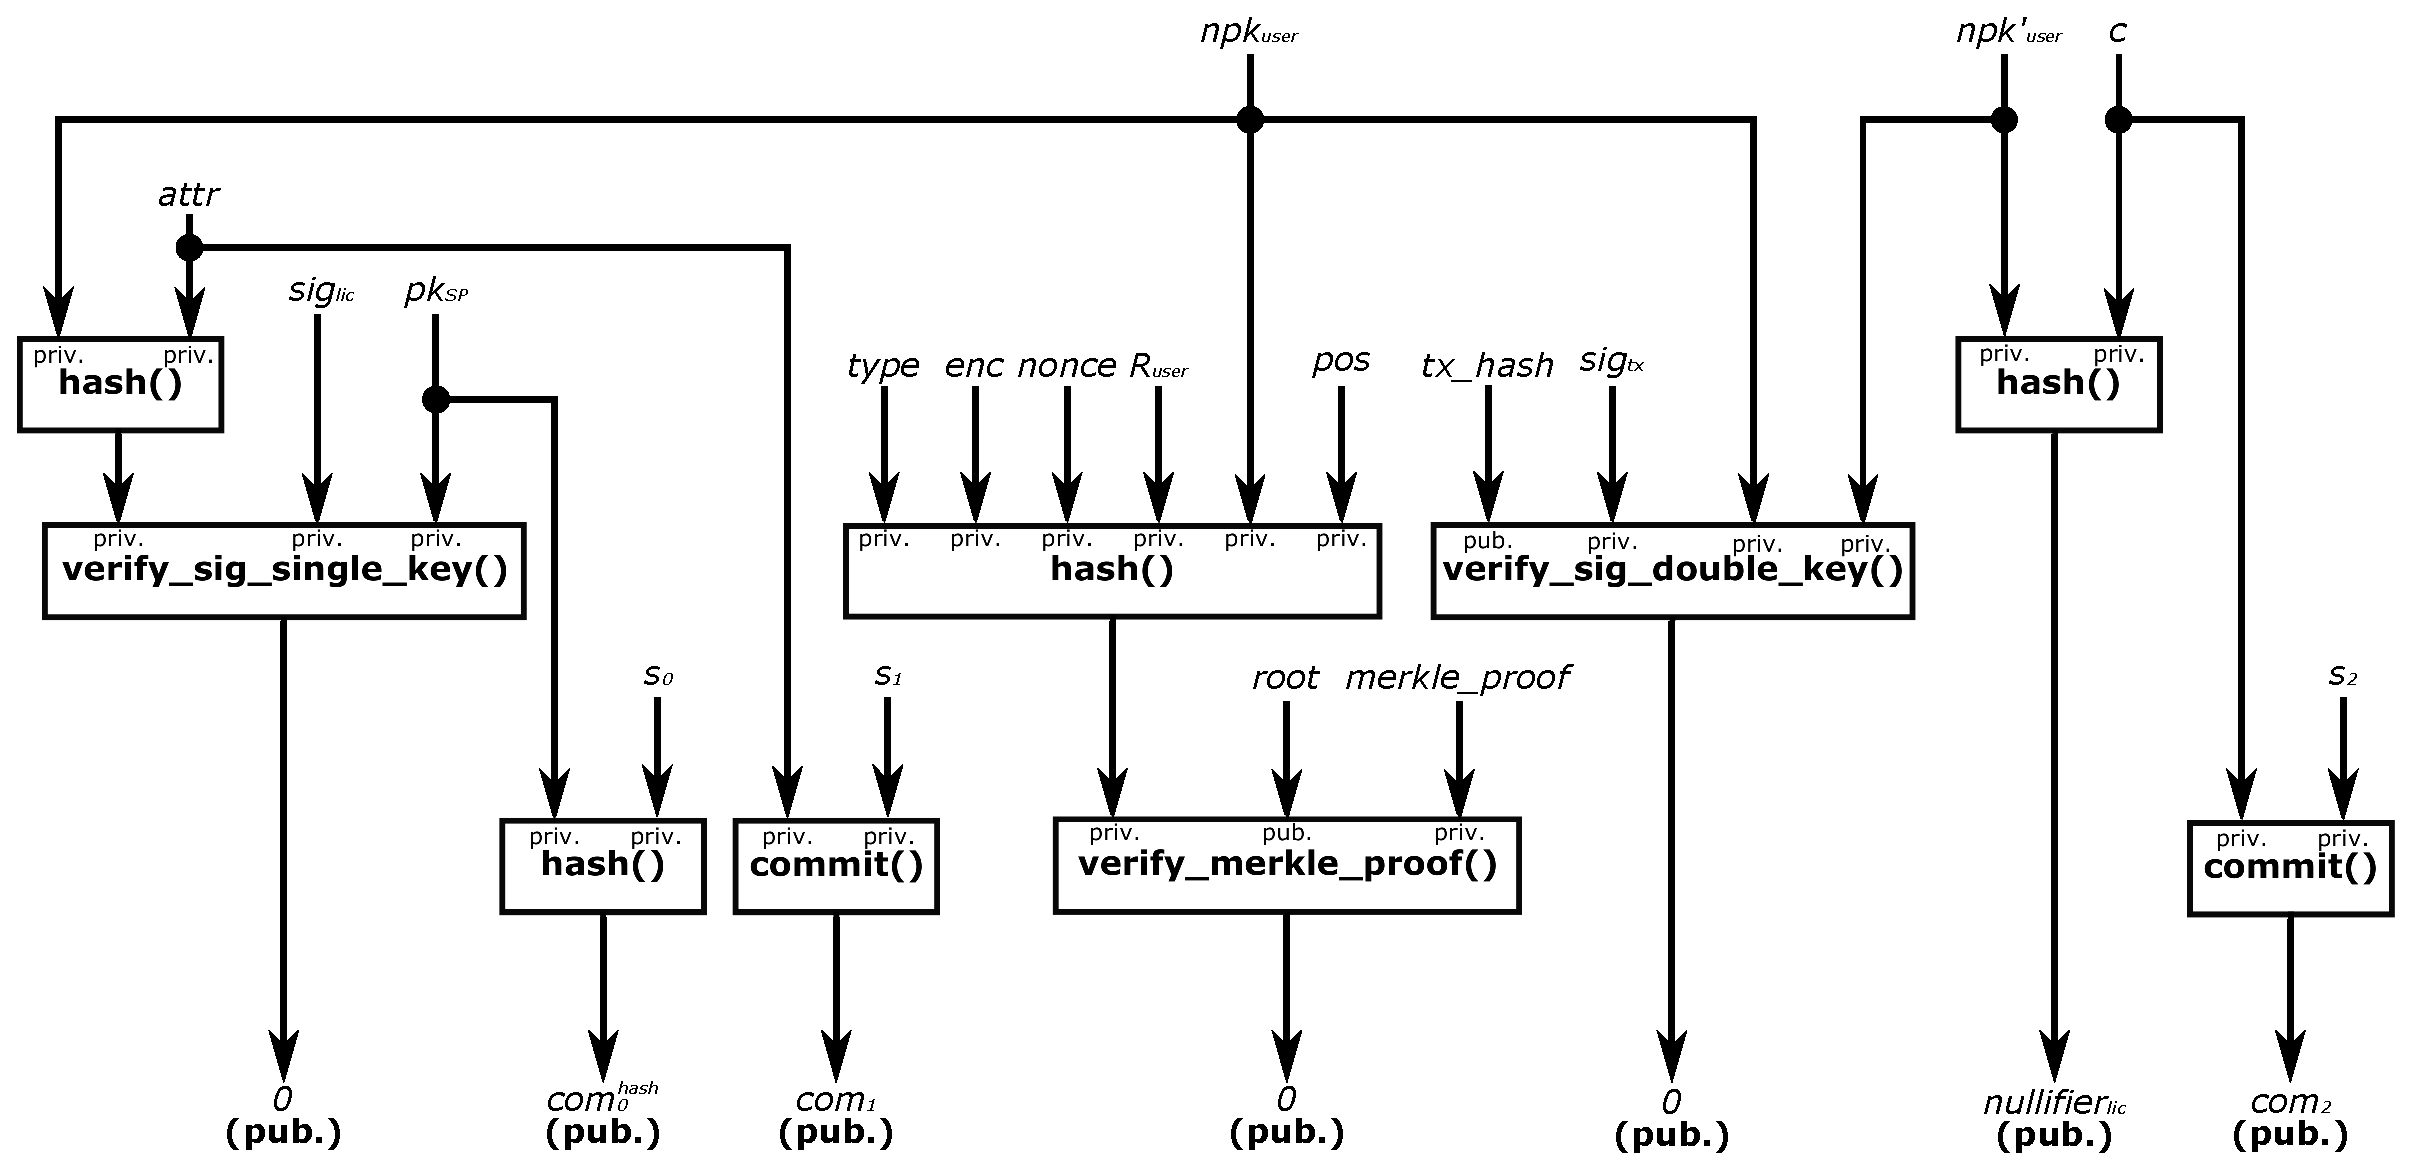
\includegraphics[width=460pt,draft=false]{images/circuit_prove_nft.eps}}
	\caption{Arithmetic circuit for proving a license's ownership.}
	\label{fig:circuit_prove_nft}
\end{figure}

As can be seen, the fact that only the user knows the $\nsk$ required to compute $\lsig$ allows them to prove ownership of the license, by means of the double key Schnorr signature, and this license is verified by proving knowledge of a valid signature verified with the public key of the SP. 

Moreover, we can appreciate in the circuit how the license is linked to the $\npk_{\user}$, and the user also verifies a Merkle proof that proves membership of this note in the Dusk Network. This brings the revocation feature: if under some circumstances the SP no longer accepts some previously issued licenses, they can prove to the network that a given note contains a license issued by them, and under a consensus agreement, it will be removed. As such, after removal, the user will not be able to provide valid proofs for this license anymore. Plus, it can happen that a user receives a license, but the transaction is finally not accepted in the Blockchain (e.g. the transaction proof was not correct, some regulation checks have failed, etc.). In this scenario, the received license will not be valid, and the user indeed will not be able to provide a correct Merkle proof.

Furthermore, the SP might request the user to nullify the license they are using (i.e. this is a single-use license, like entering a concert). This is done through the computation of $\lnullifier$. The deployment of this part of the circuit has two different possibilities:
	\begin{itemize}
		\item If we set $c = 0$ (or directly remove this input from the circuit), the license will be able to be used only once.
		\item If the SP requests the user to set a custom value for $c$ (e.g. the date of an event), the license will be able to be reused only under certain conditions.
	\end{itemize}

It is also interesting to notice that the whole protocol has been designed with perfect integration into Dusk Network. As can be noticed, all the information needed to prove ownership of a license is stored on-chain. As such, a user setting up a new instance of the Dusk wallet will be able to retrieve all the licenses by simply knowing his static secret key, as would be done with the whole Dusk protocol. The same happens with the delegation of the received notes check, where the user delegates the process of checking which notes are addressed to them. In \verb!Citadel!, the user can securely delegate the check of received licenses. Furthermore, proof delegation is also possible, as the user knowing $\nsk$ will use this key to sign a specific transaction, and this cannot be modified.

\subsubsection{Security Analysis}

We start the security analysis of \verb!Citadel! by elaborating on the ZKP scheme to use. The need for a trusted setup is one of the main drawbacks of some ZKP constructions like PlonK, especially when used in scenarios like cryptocurrencies. An untrusty setup where an adversary gets the seed used to compute it would allow them to create false transactions, and this would lead to huge losses of money. In \verb!Citadel!, an untrusted setup would lead to user impersonation, and being able to use others' licenses.

On the other hand, the soundness property of each scheme relies on different security assumptions \cite{assumptions} (e.g. the specific zk-SNARK described in \cite{cryptoeprint:2016:260} uses a strong assumption, the q-Power Knowledge of Exponent ($q$-PKE) assumption). In other words, the security of these schemes relies on the security of elliptic curves, where breaking the security of the selected curve would lead to being able to generate false proofs. In our scenario, the BLS12-381 \cite{zcash} is used. It is estimated to have around 128 bits of security, which complies with the security standards.

We now put the spotlight on the security of the circuit we have designed, which grants the following features:

\begin{itemize}
	\item \textbf{Proof of Ownership:} the circuit used in \verb!Citadel! verifies a signature $\lsig$ of an input message $(\npk_{\user}, \attr)$, using the public key of SP, $\pk_{\SP}$. Also, a double key signature $\tsig$ of a transaction hash $\mathsf{tx\_hash}$ is verified in-circuit, referring to the transaction where the ZKP will be appended.

	$\lsig$ verification ensures that the license attributes are correct, and $\tsig$ ensures that the user owns such a license, as only they can compute $\npkn{\user}$ using the note secret key and compute such a signature, while keeping all these values private, so SP cannot learn the identity of the user. An adversary would not be able to prove ownership as long as $\nsk_{\user}$ is not leaked to them. This is true under the discrete logarithm assumption.
 
	\item \textbf{Proof of Validity:} the fact that $\npk_{\user}$ is part of the signature $\lsig$, ensures that the license is assigned to a specific note of the Dusk Network, and thus, a specific user of this blockchain. The circuit verifies a Merkle proof of the NFT note containing the license, which is included in the Merkle tree of notes. This ensures that the license the user is proving ownership of has been transacted in the Dusk Network, and is a valid license at the moment of issuing the transaction. 

 	An adversary willing to successfully prove ownership of a transferred license would have to craft a new pair $(\npk_{\user}, $attr$)$ that verifies $\lsig$. This is infeasible under the discrete logarithm assumption. Furthermore, the crafted $\npk_{\user}$ would have to be a collision verifying the Merkle proof.

 \item \textbf{Unlinkability:} the user sends the one-time key pair $(\npk_{\user}, R_{\user})$ to the SP, instead of the public key $\pk$. The fact that the information about the user learned by the SP is a set of one-time values ensures that the identity of the user sending these values cannot be linked to other activities done in the network. The key $\npk_{\user}$ is computed from the value $\nsk_{\user}$, which is kept secret and used only one time. As there are no other values involved in the process that identifies the user, they cannot be linked to the user's identity. This is true as long as the user does not reuse $\nsk_{\user}$. On the other hand, $\npk_{\user} = \hb(rA)G + B$, where $r$ is sampled at random and $(A, B)$ is the user's public key. As both $\hb(rA)G$ and $B$ are only known by the user, there is no way an adversary can learn $B$, because $\npk_{\user}$ can be decomposed in many ways.

 From the point of view of the network, there is unlinkability as well: when issuing the transaction, no one is able to link the nullified license to the SP, as the $\pk_{\SP}$ is blinded by committing to this value using the \textsf{hash()} function and a random value $\mathsf{s_0}$. An adversary would not be able to learn $\pk_{\SP}$ as long as the randomness involved in the hashing process is not leaked to them. This is true assuming that the hashing function is collision-resistant. On the other hand, both $\attr$ and $c$ could leak information about the service and the user. For this reason, we commit to these values (as they are scalars instead of points, we can use the Pedersen Commitment which requires fewer constraints than the hash function). An adversary would not be able to learn $(\attr, c)$ as long as the random values involved in the commitments are not leaked to them. This is true under the discrete logarithm assumption, which holds for the Pedersen commitment.
 
 \item \textbf{Decentralized Nullification:} the circuit computes the hash of $\npkn{\user}$ and a public challenge $c$, resulting in $\lnullifier$. The format of the $c$ value could change in different scenarios. Taking the example of proving ownership of a ticket for an event, ideally, $c$ would be the date of such an event. If a function checking if a given nullifier has been previously seen, results in the equation $\isseen(\lnullifier, \pnullifiers[]) \stackrel{?}{=} 1$ holding, it means that someone already entered the event with the same license. As such, we ensure that a user cannot use the same license multiple times, nor compute valid proofs for other users. $\npkn{\user}$ is fixed in advance, as such, $\lnullifier$ will always be the same for a given public input $c$, which needs to be validated by the SP.
 
\item \textbf{Attribute Blinding:} As described previously, the user provides an opening for the commitment $\com_1$ to the SP, thus leaking the $\attr$ value. An adversary would not be able to provide a valid opening as long as the randomness involved in the commitment of $\attr$ is not leaked to them. This is true under the discrete logarithm assumption, which holds for the Pedersen commitment.

Depending on the use case, it could be desirable that the values involved in $\attr$ are kept totally or partially private. In this scenario, and as suggested in the \verb!FORT! protocol, the user could instead provide an additional proof of knowledge, proving to the SP that they know the opening of $\com_1$. As an example, a Bulletproof is a kind of ZKP allowing to prove knowledge of a value that lies within a certain range. 
 
\end{itemize}

\subsubsection{Benchmarks}

We use \verb!dusk-plonk! to code the circuit used in our solution. Like this, we get the number of constraints of its different elements and thus, the efficiency of computing (and verifying) proofs. Our circuit needs four main functions:

\begin{itemize}
 \item \textsf{hash():} we use the Poseidon hash function, which uses \textbf{977 contraints} when hashing 1 input. The amount of constraints increases depending on the number of inputs.

 \item \textsf{commit():} the Pedersen commitment requires \textbf{527 constraints}.

 \item \textsf{verify\_sig\_single\_key():} Dusk uses the Schnorr proof signature scheme over BLS12-381, which uses \textbf{3388 constraints} when using the single key version.

 \item \textsf{verify\_sig\_double\_key():} Dusk uses the Schnorr proof signature scheme over BLS12-381, which uses \textbf{6645 constraints} when using the double key version.

 \item \textsf{verify\_merkle\_proof():} the circuit needs to verify a Merkle proof. Dusk uses Merkle trees of depth 17, as such, our solution will need to compute 17 Poseidon hashes. This sums up to \textbf{17807 constraints}. 
\end{itemize}

We implemented our circuit using a total amount of \textbf{34861 constraints}. Here, we need to add the constraints needed to compute the default \textsf{tx\_proof}, which are \textbf{31486 constraints} for nullifying one note. We benchmarked both the prover and verifier using an Apple Silicon M1 CPU. The prover takes \textbf{16.232 seconds} to compute the proof, and the verifier \textbf{0.007 seconds} to verify it.

Plus, it has to be taken into account that an advantage of \verb!Citadel! is that licenses can be nullified much before being used. This means that long ZKP proving times will not have a big impact on the performance of the protocol even when using devices with low computing resources. Nonetheless, and as mentioned previously, computations can be delegated as done in the standard Phoenix model, so high-performing CPUs will compute the proofs even in less time.


